\documentclass[a4paper, twoside, openright]{report}
%\usepackage[utf8x]{inputenc}
\usepackage[a4paper,top=2cm,bottom=2cm,left=2cm,right=2cm,marginparwidth=2cm]{geometry}
\usepackage[T1]{fontenc}
\usepackage{lmodern}
\edef\restoreparindent{\parindent=\the\parindent\relax}
\usepackage[parfill]{parskip}
\restoreparindent
\usepackage{tocloft}
\usepackage{afterpage}
% \usepackage[french]{babel}
\usepackage[babel=true,kerning=true]{microtype}
\usepackage[acronym]{glossaries}
\usepackage{amssymb}
\usepackage{amsmath}
\usepackage{hyperref}
\usepackage{phonenumbers}
% \usepackage{fancyhdr}
% \pagestyle{fancy}
\usepackage[backend=biber]{biblatex}
\addbibresource{src/bibliography.bib}
\usepackage{appendix}
\usepackage{float}
\usepackage{graphicx}
\usepackage{subfig}
\usepackage{svg}
\usepackage{tikz}
\usepackage{minted}
\usepackage{color}
\usepackage{xcolor}
\usepackage{csquotes}

\setlength{\cftbeforelottitleskip}{1em}
\setlength{\cftbeforeloftitleskip}{1em}
\setlength{\cftbeforetoctitleskip}{1em}

\setlength{\cftafterlottitleskip}{1.5em}
\setlength{\cftafterloftitleskip}{1.5em}
\setlength{\cftaftertoctitleskip}{1.5em}

\newcommand{\figwidth}{15cm}

\newcommand\blankpage{
    \null
    \thispagestyle{empty}
    \addtocounter{page}{-2}
    \newpage}

\newcommand\emptypage{
    \null
    \newpage}

% Command to create a glossary entry with correspondent acronym.
% https://tex.stackexchange.com/questions/8946/how-to-combine-acronym-and-glossary
% Args : 1: entry, 2: acronym/name, 3: long name, 4: description
\newcommand{\newglossaryentrywithacronym}[4]{
    %%% The glossary entry the acronym links to   
    \newglossaryentry{#1_gls}{
        name={#2},
        long={#3},
        description={#4}
    }

    % Acronym pointing to glossary
    \newglossaryentry{#1}{
        type=\acronymtype,
        name={#2},
        description={#3},
        see=[Glossary:]{#1_gls}
    }
}

\definecolor{LightGray}{gray}{0.9}

\newminted[pythonCode]{python}{
    frame=lines,
    framesep=2mm,
    baselinestretch=1.2,
    bgcolor=LightGray,
    fontsize=\footnotesize,
    linenos}

\newminted[outputCode]{bash}{
    frame=lines,
    framesep=2mm,
    baselinestretch=1.2,
    bgcolor=LightGray,
    fontsize=\footnotesize,
    linenos}

% \setlength{\headheight}{28pt}
% \fancyhead[L]{ALLEMAND Fabien}
% \fancyhead[C]{}
% \fancyhead[R]{\includegraphics[scale=0.025]{/home/fabien/logo_TSP_1.jpg}}
% \fancyfoot[L]{}
% \fancyfoot[R]{}

\makeglossaries

\newacronym{lic}{LIC}{Learned Image Compression}
\newacronym{clic}{CLIC}{Challenge on Learned Image Compression}
\newacronym{psnr}{PSNR}{Peak Signal to Noise Ratio}

% \newglossaryentry{front_end}
% {
%         name={front end},
%         description={}
% }


\begin{document}

\thispagestyle{empty}
\begin{center}

\vspace*{2.5cm}

{\fontsize{30}{30}\selectfont PRIM Project}

\rule{\textwidth}{1pt}

\medskip

{\fontsize{22}{22}\selectfont Learned Image Compression on FPGA}

{\fontsize{18}{18}\selectfont Intermediate Report}

\rule{\textwidth}{1pt}

\medskip

{\fontsize{18}{18}\selectfont Supervisors: Attilio Fiandrotti, Alaa Mazouz, Sumanta Chaudhuri}

\medskip

{\fontsize{18}{18}\selectfont Student: Fabien ALLEMAND}

\medskip

{\fontsize{14}{14}\selectfont 2024 - 2025}

\vspace*{2.5cm}

\includegraphics[height=4cm]{/home/fabien/logo_TSP_3.png}

\vfill

\end{center}

\afterpage{\blankpage}

\newpage
\pagenumbering{roman}

% \input{src/contact.tex}

% \chapter*{Acknowledgments}
Working on a six-month research project at the Institut Polytechnique de Paris has been an enriching experience, marked by numerous technical discoveries. I would like to express my gratitude to everyone who has supported and guided me throughout the project and in the writing of this report.

First and foremost, I would like to thank my supervisors, Attilio Fiandrotti, Alaa Mazouz, and Sumanta Chaudhuri, researchers at the Institut Polytechnique de Paris, for their warm welcome, the valuable time spent together, and the knowledge they shared with me.

I would also like to extend my sincere thanks to Alaa Mazouz, who directly supervised my work and collaborated with me throughout the project. His ongoing support and detailed explanations were crucial in helping me understand the tasks entrusted to me and in acquiring new skills that will undoubtedly benefit my future endeavors.

\printglossary[type=\acronymtype]
\printglossary

% \newpage
%\listoftables

% \afterpage{\emptypage}

\newpage
\listoffigures

\afterpage{\emptypage}

\newpage
\tableofcontents

\afterpage{\emptypage}

\newpage
\pagenumbering{arabic}

\chapter*{Introduction}
\addcontentsline{toc}{chapter}{Introduction}
Since the beginning of computers, the amount of raw data has always exceeded the capacity of storage mediums. With the quantity of created data approaching 500 terabytes every day in 2024, data compression has become ubiquitous. Whether it is to improve storage capacity or enhance data transfer, data compression is used regardless of the scale. Let us focus on image data. Image files on a computer disk can be compressed to take less storage space. Video streams of data transfered over the internet are compressed in order to make transfers more efficient in terms of resource availability and energy consumption. Both examples highlight the induced improved user experience (ability to store more files on the same disk and fast download speeds).

However data compression comes at a cost. There is a limit to how many bits can be removed while encoding the exact same data. Past this limit, some data is lost which can degrade the content of the file to various degrees. This process, called lossy image compression (as opposed to lossless compression), introduces a tradeoff between data compression and data quality. There is a wide variety of (deterministic) algorithms used to compress data. Some of them are designed to focus on compression at the cost of quality. Such algorithms (like GIF) work well for simple schematics and diagrams but introduce artifacts on more complex files like photographs. State of the art algorithms (like JPEG or Webp) manage to perform data compression while preserving the majority of the file content. Some artifacts can be added but they can be negligeables depending of the use case (for instance they are often not visible to the human eye without close inspection).

With the recent progress of machine learning, new compression algorithms appeared. These probabilistic algorithms are based on neural networks that can learn a better way to encode data with a minimum number of bits. The only issue being that these methods require way more processing power than previous state of the art compression algorithms. The goal of this project is to achieve real-time image compression on resource constrained platforms. Chapter \ref{sota} summarises state of the art methods. The first results achieved in the context of this project mainly consist in reproducing state of the art results and are presented in Chapter \ref{results}.
% Section \ref{lic} explains how machine learned image compression works and Section \ref{sota} briefly presents state of the art methods. Finally, ... of this project is shown in Section \ref{results}.

\chapter{Learned Image Compression}
\label{lic}

\chapter{State of the Art}
\label{sota}
\acrfull{lic} is a lossy compression method based on machine learning. Using autoencoder architecture, it is possible to build and train end-to-end a neural network that achieves balance between image compression efficiency and reconstruction fidelity. \acrshort{lic} consists of three successive steps: projection in a low-dimensional latent space (using the encoder part of the autoencoder), quantisation and lossless entropy coding. Decompression is achieved by applying entropy decoding and projecting the result back into the image space with the decoder part of the autoencoder \cite{licmedium, licstanford}.

Early seminal works accounted for a unique latent representation modelled with a fully factored distribution \cite{ballé2017endtoendoptimizedimagecompression}. Since then, much of the research in the field has focused on improving the compression efficiency by refining the entropy model. This basic scheme was then improved by introducing an auxiliary latent space called hyperprior capturing spatial correlation within the image, furthering compression efficiency \cite{ballé2018variationalimagecompressionscale}. \acrshort{lic} has shown the ability to outperform standardised video codecs in compression efficiency, fostering the demand for embedded hardware implementations.

Applying frugal machine learning techniques can help reducing the load of the neural network on the computer. Such methods include pruning, quantisation or knowledge distillation \cite{touvron2021trainingdataefficientimagetransformers}. It should be noted that knowledge distillation can be achieved between different architecture opening the possibility to use a completely different network for decoding \cite{liu2022crossarchitectureknowledgedistillation}.

Achieving real-time coding on resource constrained platforms such as FPGAs demands ad-hoc design choices such as in the state of the art \acrshort{lic} implementations. However, FPGA implementations have been lagging behind recent research in \acrshort{lic} due to the increasing complexity of implementing in hardware recent \acrshort{lic} models. For example, further improves the RD efficiency by introducing slice-based latent channel conditioning and latent residual prediction with an approach suitable for parallel execution. The RD efficiency is further boosted in the work of Zou et al. \cite{zou2022devildetailswindowbasedattention} by introducing a Window Attention Module in the autoencoder architecture and experimenting with a transformer-based architecture in place of the traditional convolutional architecture.

\chapter{Results}
\label{results}
This chapter presents the results achieved during the first part of this project. In a first part, we introduce the tools we use (libraries, datasets). A second part describes our methodology and results regarding the reproduction of state of the art.

\section{Methodology}
As explained in chapter \ref{sota}, state of the art \acrshort{lic} models provide great results: they provide encoding of images that contain very few bits while preserving the images quality. However, these models require a lot of processing power making them unsuitable for realtime application on resource constrained devices. The goal of this project is to explore solutions to reduce the processing power used by these models, leading to realtime image compression/decompression on such devices. In order to do that, it is necessary to have access to the state of the art \acrshort{lic} models, the image datasets used to train them and enough processing power to train such models.

CompressAI \cite{compressai} is a Python library for learned compression. Based on the well known machine learning library PyTorch, compressAI provides custom operations, layers and models for deep learning based data compression and pre-trained end-to-end compression models for \acrshort{lic}. Amongs the pre-trained models is the model from Ballé et al.\cite{ballemshj18} that will be used throughout the project.

Usually, researchers train their models on the OpenImages dataset \cite{openimages} but pre-trained models on compressAI have been trained on the Vimeo90K dataset \cite{xue2019video}. In order to perform proper model comparisons, the Vimeo dataset will be used for training in this project. For testing, two datasets will be used: the Kodak dataset \cite{kodak} and the dataset from the \acrfull{clic} \cite{clic}.

The computing power required for training and using models will be provided by the GPU cluster of Télécom Paris.

\section{Results Reproduction}
In a research project, reproducing state of the art results is key. The first thing to do is to ensure that our work environnement is correct by reproducing results from articles. This also provides a shared baseline results between papers and our work, that can be used to compare our future results.

As experiments parameters are not disclosed in the papers we studied, we try to reproduce results from the compressAI library, taht is to say: achieve the same results as the pre-trained models from the model zoo.

The training methodology used by compressAI is described in the documentation \cite{compressai_train}. Models were trained between 4 and 5 million steps on 256x256 image patches randomly extracted and cropped from the Vimeo90K dataset. The batch size is 16 or 32 (we choose 16). The initial learning rate is 1e-4 and decreases over time (it is divided by 2 when the evaluation loss reaches a plateau). Two different metrics can be used: MSE or MS-SSIM. We keep the default metric (MSE) which corresponds to using the following loss function: \(L = \lambda * 255^{2} * D + R\) with \(D\) and \(R\) respectively the mean distortion and the mean estimated bit-rate. The parameter \(\lambda\) allows to adjust the tradeoff between compression and image quality. Higher values give more importance to distortion encouraging the model to produce reconstructed images with high quality at the expense of bit-rate. Inversely, lower values of \(\lambda\) imply more compression and more data loss. CompressAI proposes 8 pre-trained models with different values of \(\lambda\) represented by the argument \textsf{quality}. The correspondance between this argument and the value of \(\lambda\) is summarised in Table \ref{tab}. It is important to note that the \textsf{quality} argument in compressAI also impacts the network architecture.

\begin{table}[]
    \centering
    \begin{tabular}{|l|c|c|c|c|c|c|c|c|}
    \hline
    \textsf{quality}                      & 1 & 2 & 3 & 4 & 5 & 6 & 7 & 8 \\ \hline
    Value of \(\lambda\) for MSE & 0.0018 & 0.0035 & 0.0067 & 0.0130 & 0.0250 & 0.0483 & 0.0932 & 0.1800 \\ \hline
    \end{tabular}
    \caption{Correspondance between the argument \textsf{quality} in compressAI and the value of \(\lambda\) when using MSE}
    \label{tab}
\end{table}

This part of the project is divided in two parts. First, we try to train a single model and compare it to other pre-trained models. Then we train several models in order to produce rate-distortion curves.

\subsection{Single Model}
Using the training script provided by compressAI and following the same methodology, we train a model for \(5 \times 24\) hours (approximately 700 epochs). Eventhough weights are loaded from previous checkpoint at the beginning of each training, this is different than training the model for 6 hours straight due to the change of learning rate over time (for each training session the learning rate is set back to 1e-4). We use the default value for \(\lambda\) (1e-2) and the architecture corresponds to setting the compressAI argument \textsf{quality} to 3.

After training we can evaluate our model. First, we try a single inference with this newly trained model. Figure \ref{balle_repro_1} shows that the reconstructed image (middle) is visually close to the original image. However, the difference between the two images (right) reveals that there are a lot of differences. These differences are compared in the part of the image that contains details. These parts are often refered as containing high frequencies an are particularly hard to compress as opposed to low frequency areas (like the sky in this picture) that do not contain a lot of information and are easier to compress.

\begin{figure}
    \centering
    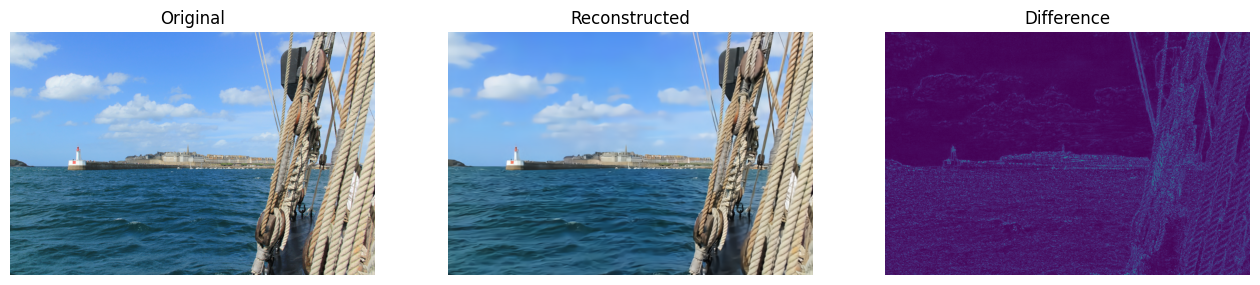
\includegraphics[width=15cm]{img/balle_repro_1.png}
    \caption{Comparison of the reconstrcuted with the original image}
    \label{balle_repro_1}
\end{figure}

Figure \ref{balle_repro_2} shows encoding of the image at the same bit-rate using different methods. It is clear that the network is the more accurate among the three methods used: the reconstructed image is closer to the original image. JPEG introduces a lot of artifacts (blocs) and Webp does not retains as much details as the network, especially in the water.

\begin{figure}
    \centering
    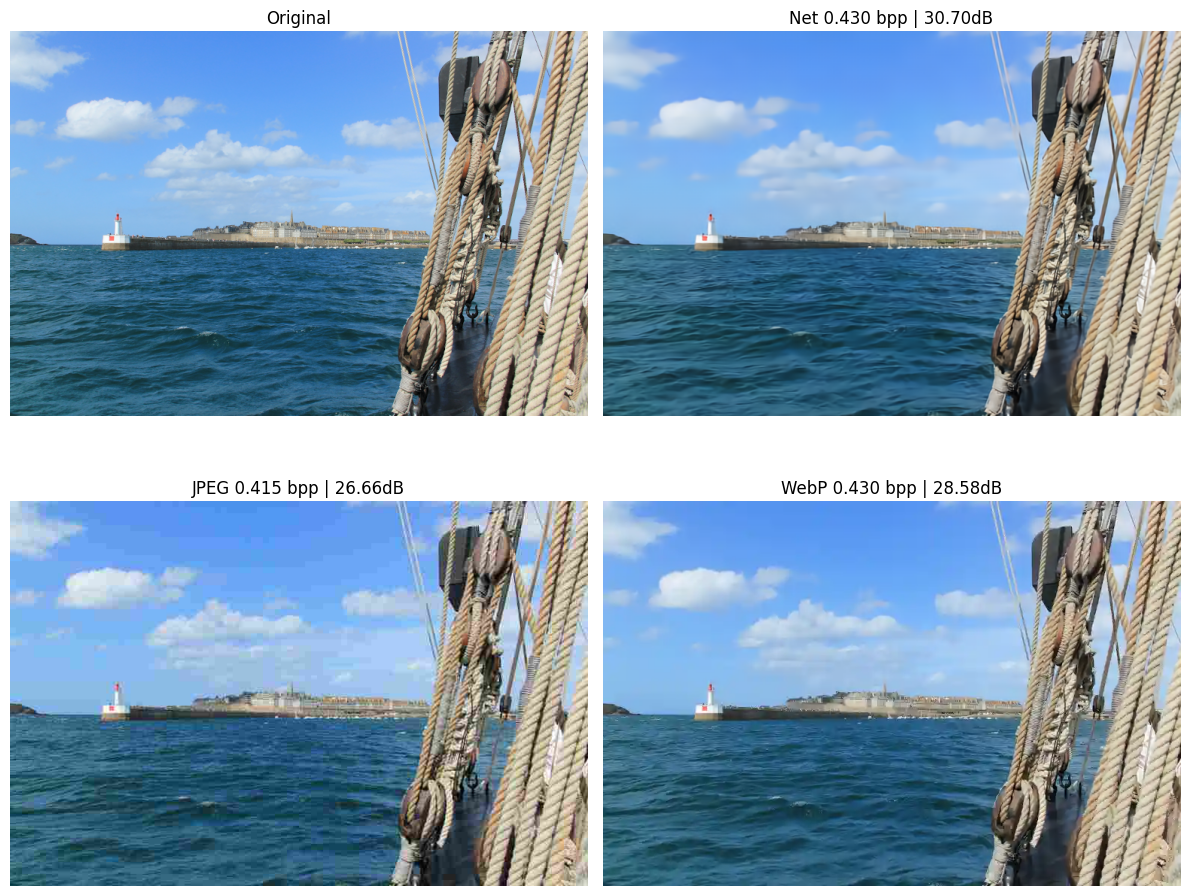
\includegraphics[width=15cm]{img/balle_repro_2.png}
    \caption{Comparison to classical codecs: quality coparison at similar bit-rate}
    \label{balle_repro_2}
\end{figure}

For the same distortion rate, our model manages has the smallest bit-rate out of the three methods, that is to say: for the same visual quality, measured by the \acrful{psnr}, the image is more compressed. Figure \ref{balle_repro_3} shows that it achieves less than 0.5 bits per pixel whereas traditional compression methods like Webp or JPEG achieve respectively 0.698 and 1.054 bit per pixels.

\begin{figure}
    \centering
    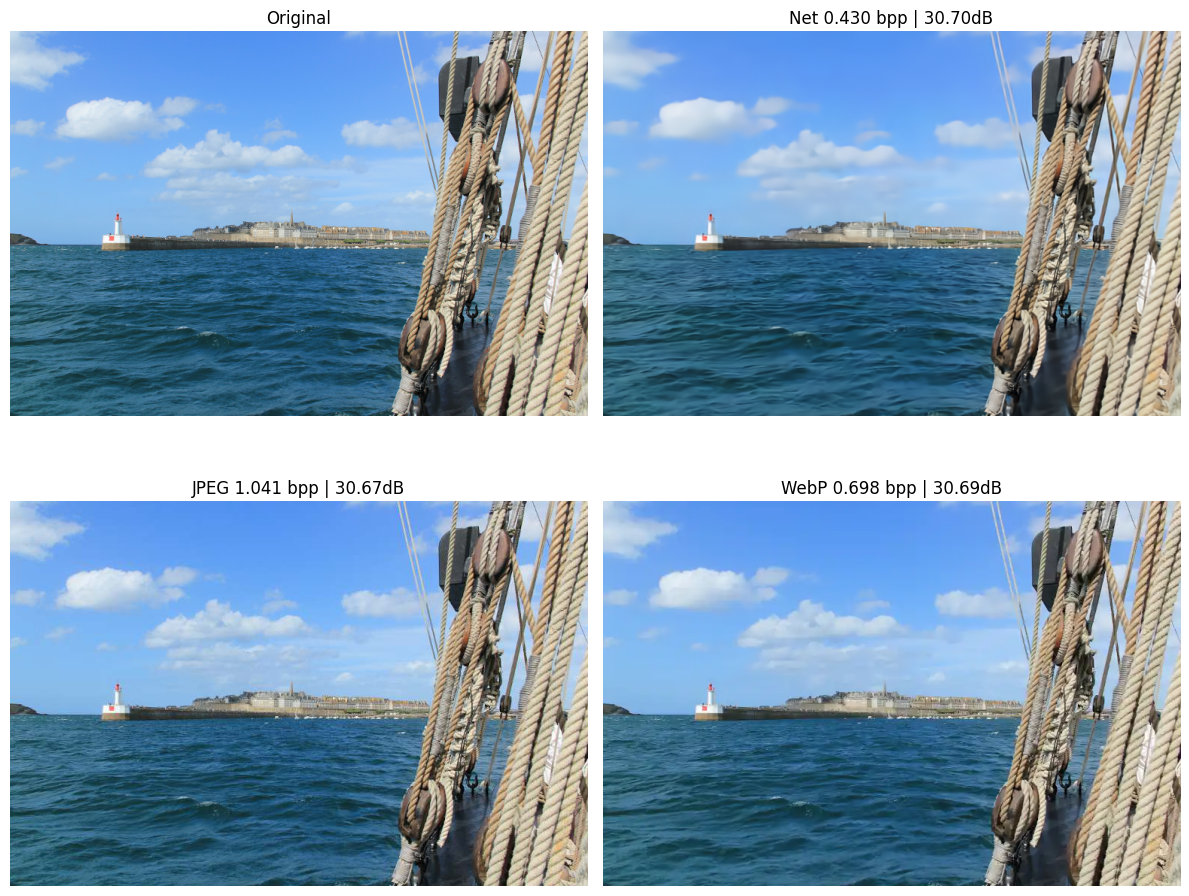
\includegraphics[width=15cm]{img/balle_repro_3.png}
    \caption{Comparison to classical codecs: bit-rate coparison at similar PSNR}
    \label{balle_repro_3}
\end{figure}

Similar results are observed on Figure \ref{balle_repro_4} which is based on MS-SSIM, another method to measure visual fidelity.

\begin{figure}
    \centering
    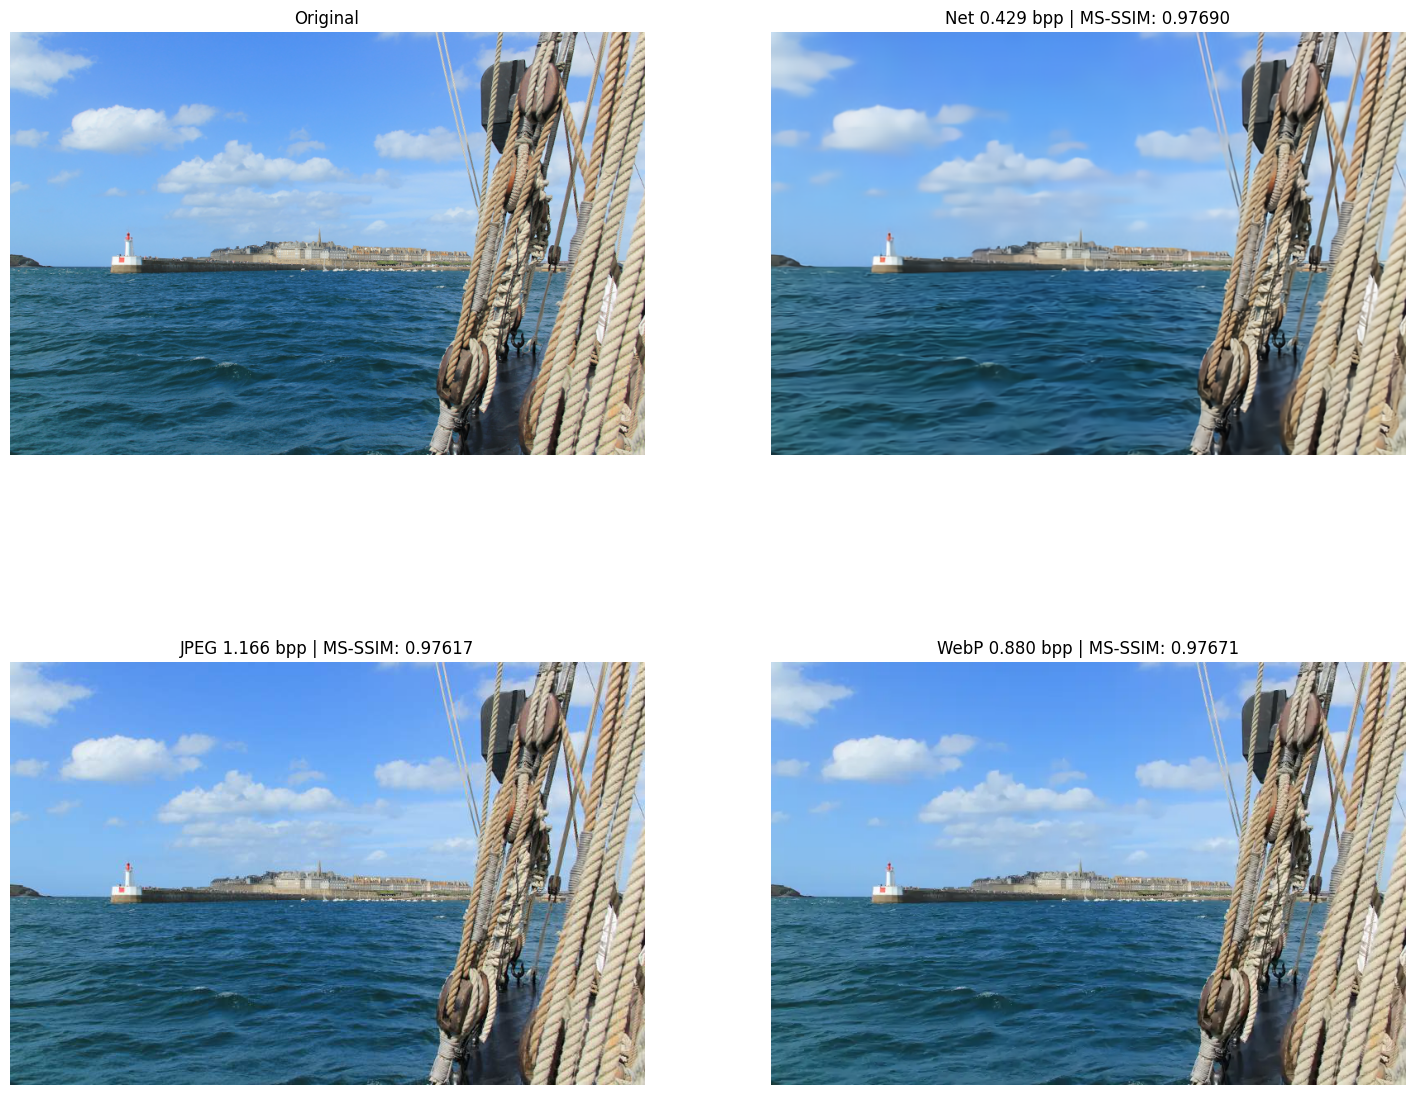
\includegraphics[width=15cm]{img/balle_repro_4.png}
    \caption{Comparison to classical codecs: bit-rate coparison at similar MS-SSIM}
    \label{balle_repro_4}
\end{figure}

Finally, we compare our models to other \acrshort{lic} models accessbible in the compressAI model zoo. Figure \ref{balle_repro_5} allows to compare visual results from our model at three stages of the training and various pre-trained models. Results are visually close but, by zooming, it is clear that our models retain more details than the other pre-trained models (for intance in the ropes). This is coherent with Figure \ref{balle_repro_6} that shows that our models are more focused on quality at the expense of bit-rate (located in the top right of the plot). Other models perform worse in term of image quality but achieve a lower compression rate (bottom left of the plot).

\begin{figure}
    \centering
    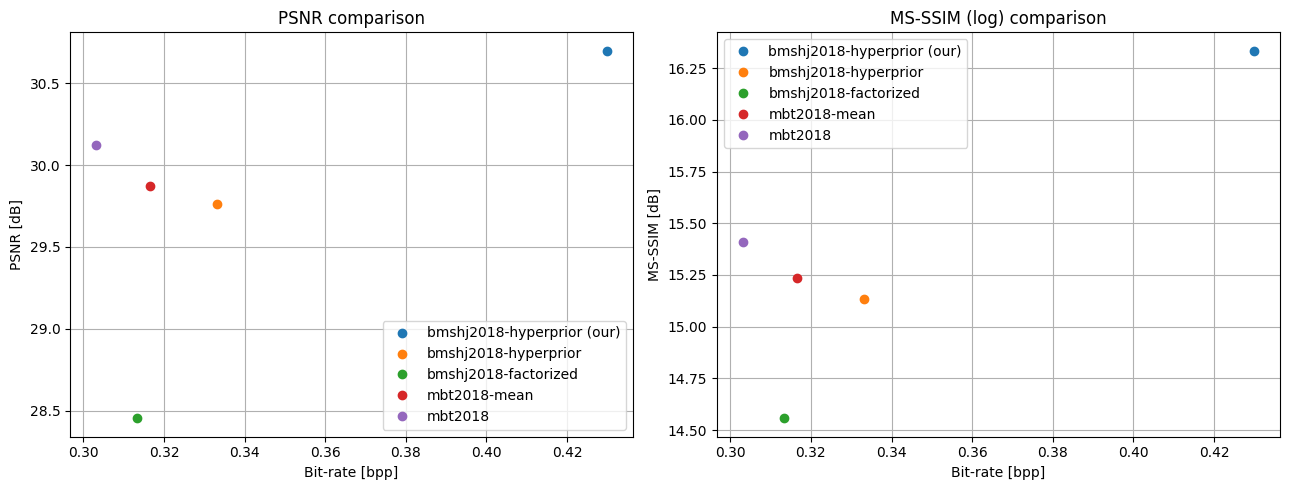
\includegraphics[width=15cm]{img/balle_repro_5.png}
    \caption{Comparison to other \acrshort{lic} models: image reconstruction}
    \label{balle_repro_5}
\end{figure}

\begin{figure}
    \centering
    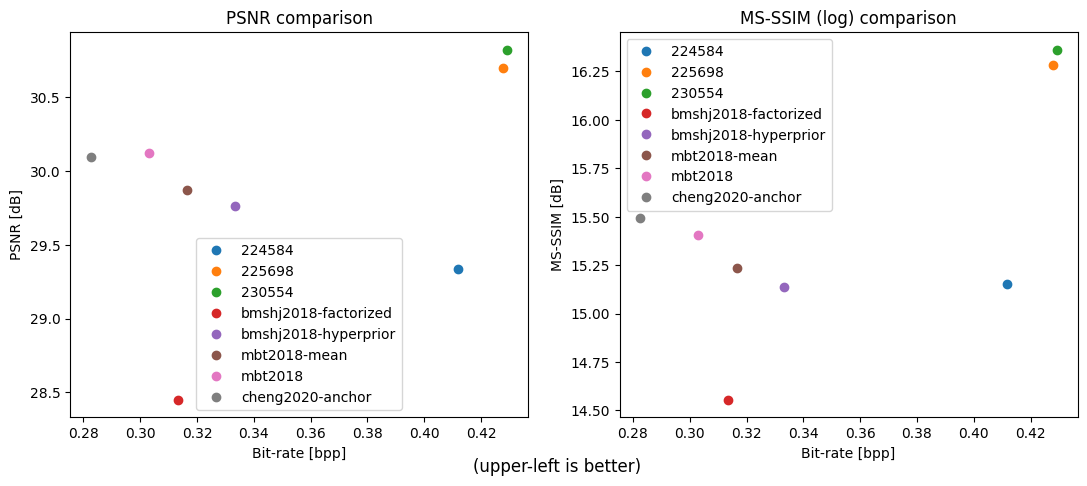
\includegraphics[width=15cm]{img/balle_repro_6.png}
    \caption{Comparison to other \acrshort{lic} models: rate-distortion curves}
    \label{balle_repro_6}
\end{figure}

This section show that we are able to train a \acrshort{lic} model that can compress and reconstruct images while mostly preserving its content. Our models perform better than deterministic codecs like JPEG or Webp but our models does not produce the same results as the pre-trained ones. It should be noted that, at this point, we are mainly checking if training is working properly on the GPU cluster and that we are now comparing models that were trained differently. Next section focuses more on the models parameters and the impact on the bit-rate/distortion tradeoff.

\subsection{Rate-Distortion Curves}
Using the training script provided by compressAI and following the same methodology, we train 8 different models: one for each value of \textsf{quality}. That is to say, one for each couple of \(\lambda\) value and corresponding model architecture. However, to quickly achieve comparable results, we limit the number of epochs to 65, just under what the GPU cluster is able to compute in 24 hours.

This method allows us to compare models more precisely by taking into account the bit-rate/distortion tradeoff induced by the value of \(\lambda\) parameter. Figure \ref{bdpsnr_1} and \ref{bdpsnr_2} show image reconstruction results from our models and pre-trained models for each value of \(\lambda\). There is a clear change in image quality between images in the top-left corresponding to lower values of \(\lambda\) (low bit-rate and low quality) and images in the bottom-right corner correponding to higher values of \(\lambda\) (high bit-rate and high quality) for both our models and pre-trained models.

\begin{figure}[H]
    \centering
    \subfloat[Our networks]{{\includegraphics[width=8.5cm]{../bdpsnr/test_res/20241129_085637/networks_kodak_kodim14.png} \label{bdpsnr_1:a}}}
    \subfloat[Pre-trained networks]{{\includegraphics[width=8.5cm]{../bdpsnr/test_res/20241129_085637/pretrained_networks_kodak_kodim14.png} \label{bdpsnr_1:b}}}
    \caption{Reconstruction results on image 14 of the Kodak dataset}
    \label{bdpsnr_1}
\end{figure}

\begin{figure}[H]
    \centering
    \subfloat[Our networks]{{\includegraphics[width=8.5cm]{../bdpsnr/test_res/20241129_085637/networks_kodak_kodim15.png} \label{bdpsnr_2:a}}}
    \subfloat[Pre-trained networks]{{\includegraphics[width=8.5cm]{../bdpsnr/test_res/20241129_085637/pretrained_networks_kodak_kodim15.png} \label{bdpsnr_2:b}}}
    \caption{Reconstruction results on image 15 of the Kodak dataset}
    \label{bdpsnr_2}
\end{figure}

We are also able to produce rate-distortion curves for each image of the testing dataset in order to compare our models with pre-trained models. Figure \ref{bdpsnr_3} show an example of one of this curve. This shows that for lower bit-rate (lower values of \(\lambda\)) our model is very similar to the pre-trained models but there is a slight difference for higher bit-rates where our models do not reach the same level of image quality.

\begin{figure}
    \centering
    \includegraphics[width=15cm]{../bdpsnr/test_res/20241129_085637/curve_kodak_kodim15.png}
    \caption{Rate-distortion curve for image 14 of the Kodak dataset}
    \label{bdpsnr_3}
\end{figure}

By averaging metrics on the test dataset, we create an average rate-distortion curve for the entire test dataset. This curve is shown in Figure \ref{bdpsnr_4}. Results are similar to those obtained in Figure \ref{bdpsnr_3}: our models are very close to pre-trained models with a little disadvantage when dealing with higher bit-rates.

\begin{figure}
    \centering
    \includegraphics[width=15cm]{../bdpsnr/test_res/20241129_085637/avg_curve_kodak.png}
    \caption{Average rate-distortion curve for the Kodak dataset}
    \label{bdpsnr_4}
\end{figure}

These results show that we are able to reproduce state of the art results for \acrshort{lic} using publicly available datasets and the processing power of the Télécom Paris GPU cluster.

\section{Future Work}
Current results prove that we are able to achieve close to, if not state of the art \acrshort{lic} results on traditional hardware. Future work will focus on improving models to work on power constrained platforms (like FPGA) by using techniques like pruning, quantisation and knowledge distillation. We will start by implementing and evaluating these techniques to work on single images whereupon we will add the realtime constraint.

\chapter*{Conclusion}
\addcontentsline{toc}{chapter}{Conclusion}
Data compression and especially image compression is a crucial tool in information technology. Whether it is to save storage space or to improve networks efficiency, the goal is to represent the same information with the minimum amount of bits. Lossless compression is limited, leaving place to lossy compression. This compression method introduces a tradeoff between storage space and data quality/integrity.

Using existing deep learning and computer vision tools, \acrfull{lic} aims to provide a new way to perform image compression providing better results than previous deterministic codecs. \acrshort{lic} requires a lot of processing power making it unsusable on resource constrained platforms.

The final goal of this project is to explore technique allowing to use \acrshort{lic} on these low power devices possibly in real-time. After reproducing state of the art results, the goal is to explore frugal machine learning techniques such as pruning, quantisation and knowledge distillation.

\printbibliography

\appendix

\chapter{Reproducibility}

\section{Implementation Details}
Here is a list of useful details regarding our implementation:
\begin{itemize}
    \item Python 3.12.7
    \item Anaconda virtual environment
    \item compressAI 1.2.6
    \item Code hosted on private GitHub repository
    \item Processing power provided by Télécom Paris GPU cluster (\url{https://docs.google.com/document/d/1lXykfpEUJCrbNh22D2f2kxNS0gV6t-j9A_juWFdiEnI/edit?tab=t.0})
\end{itemize}

\section{Measures}

% TODO

\chapter{Figures}

\begin{figure}
    \centering
    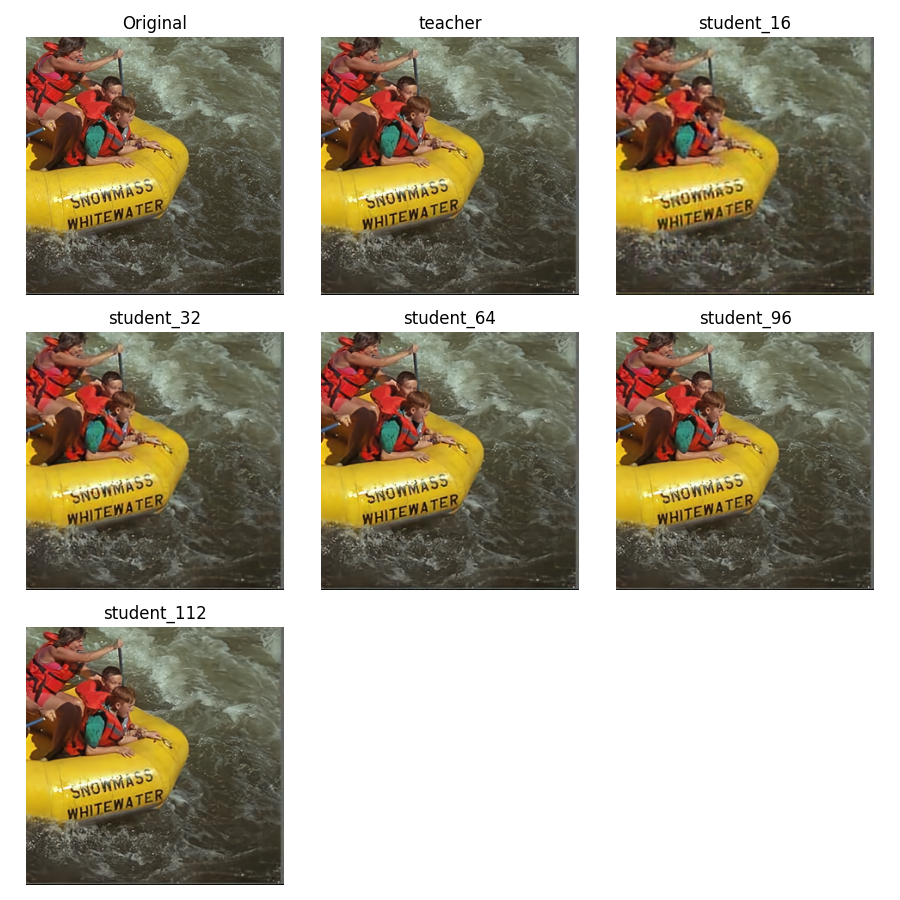
\includegraphics[width=15cm]{img/kd_ae_kodak_14.png}
    \caption[Evaluation on the Kodak dataset of the scale hyperprior student models trained for image compression: reconstruction results on image 14 of the Kodak dataset with teacher and student architectures.]{Evaluation on the Kodak dataset of the scale hyperprior student models trained for image compression: reconstruction results on image 14 of the Kodak dataset with teacher and student architectures.}
    \label{appendix:kd_ae_1}
\end{figure}

\begin{figure}
    \centering
    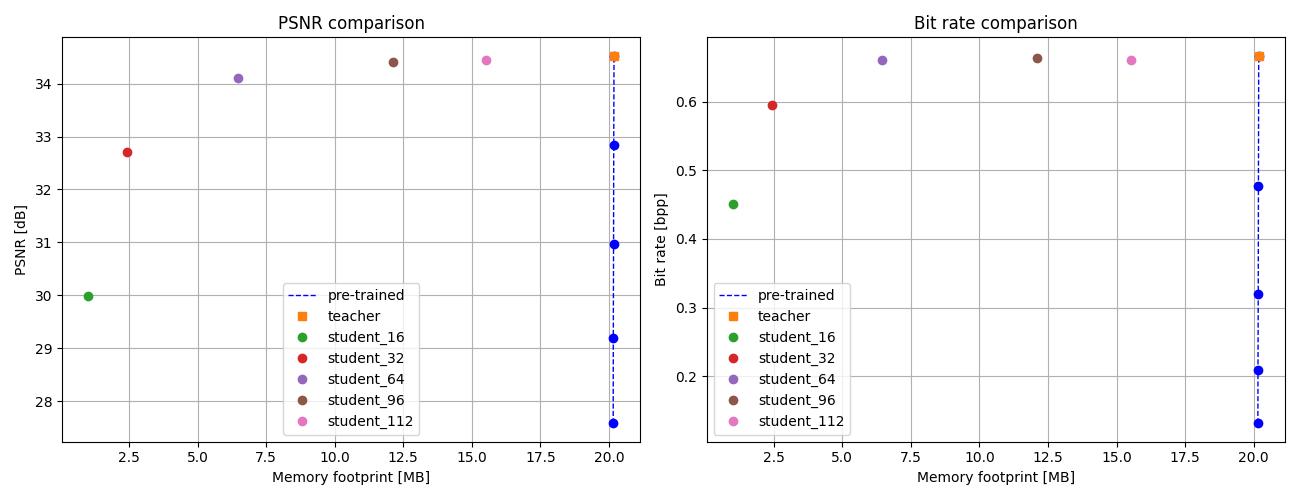
\includegraphics[width=15cm]{img/kd_lic_memory.png}
    \caption[\acrshort{psnr} and bit rate on the Kodak dataset according to students memory footprint.]{\acrshort{psnr} and bit rate on the Kodak dataset according to students memory footprint.}
    \label{appendix:kd_lic_memory}
\end{figure}

\begin{figure}
    \centering
    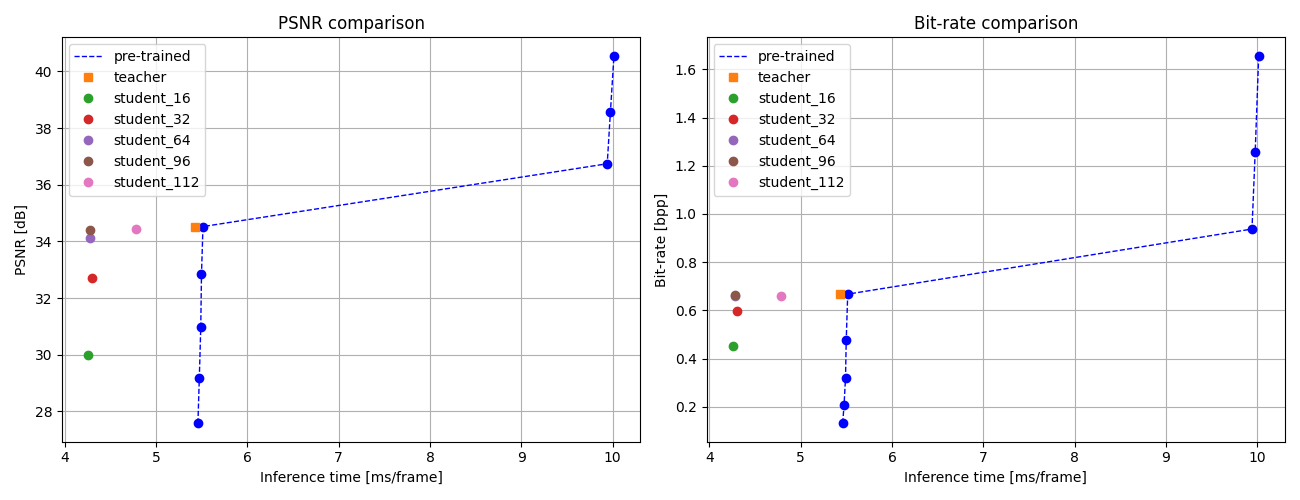
\includegraphics[width=15cm]{img/kd_lic_time.png}
    \caption[\acrshort{psnr} and bit rate on the Kodak dataset according to students inference time.]{\acrshort{psnr} and bit rate on the Kodak dataset according to students inference time.}
    \label{appendix:kd_lic_time}
\end{figure}

\begin{sidewaystable}[]
    \centering
    \begin{tabular}{|c|c|lr|lr|lr|lr|lr|lr|lr|}
        \hline
        Model                     & \begin{tabular}[c]{@{}c@{}}Number\\ of channels\end{tabular} & \multicolumn{2}{c|}{\begin{tabular}[c]{@{}c@{}}Number of\\ parameters {[}M{]}\end{tabular}} & \multicolumn{2}{c|}{\begin{tabular}[c]{@{}c@{}}Memory\\ footprint {[}MB{]}\end{tabular}} & \multicolumn{2}{c|}{\begin{tabular}[c]{@{}c@{}}Floating point\\ operations\\ {[}GFLOP/frame{]}\end{tabular}} & \multicolumn{2}{c|}{\begin{tabular}[c]{@{}c@{}}Throughput\\ {[}FPS{]}\end{tabular}} & \multicolumn{2}{c|}{\begin{tabular}[c]{@{}c@{}}Energy\\ {[}mJ/frame{]}\end{tabular}} & \multicolumn{2}{c|}{PSNR}               & \multicolumn{2}{c|}{\begin{tabular}[c]{@{}c@{}}Bit rate\\ {[}bpp{]}\end{tabular}}      \\ \hline
        Teacher                   & 128                        & {\color[HTML]{656565} }                                  & 5.08                         & {\color[HTML]{656565} }                                  & 20.18                        & {\color[HTML]{656565} }                                  & 34.24                        & {\color[HTML]{656565} }                                  & 184.20                         & {\color[HTML]{656565} }                                  & 1767.85                         & {\color[HTML]{656565} }                                 & 34.53                         & {\color[HTML]{656565} }                                 & 0.67                         \\ \hline
                                  & 112                        & {\color[HTML]{656565} -19.77 \%}                         & 4.07                         & {\color[HTML]{656565} -23.03 \%}                         & 15.53                        & {\color[HTML]{656565} -22.01 \%}                         & 26.70                        & {\color[HTML]{656565} +13.47 \%}                         & 209.01                         & {\color[HTML]{656565} -9.47 \%}                          & 1600.41                         & {\color[HTML]{656565} -0.26 \%}                         & 34.44                         & {\color[HTML]{656565} -1.03 \%}                         & 0.66                         \\ \cline{2-16} 
                                  & 96                         & {\color[HTML]{656565} -37.47 \%}                         & 3.17                         & {\color[HTML]{656565} -40.01 \%}                         & 12.11                        & {\color[HTML]{656565} -41.31 \%}                         & 20.10                        & {\color[HTML]{656565} +25.74 \%}                         & 231.61                         & {\color[HTML]{656565} -19.88 \%}                         & 1416.34                         & {\color[HTML]{656565} -0.33 \%}                         & 34.41                         & {\color[HTML]{656565} -0.58 \%}                         & 0.66                         \\ \cline{2-16} 
                                  & \cellcolor[HTML]{EFEFEF}64 & \cellcolor[HTML]{EFEFEF}{\color[HTML]{656565} -66.62 \%} & \cellcolor[HTML]{EFEFEF}1.69 & \cellcolor[HTML]{EFEFEF}{\color[HTML]{656565} -67.98 \%} & \cellcolor[HTML]{EFEFEF}6.46 & \cellcolor[HTML]{EFEFEF}{\color[HTML]{656565} -71.75 \%} & \cellcolor[HTML]{EFEFEF}9.67 & \cellcolor[HTML]{EFEFEF}{\color[HTML]{656565} +26.20 \%} & \cellcolor[HTML]{EFEFEF}232.47 & \cellcolor[HTML]{EFEFEF}{\color[HTML]{656565} -34.15 \%} & \cellcolor[HTML]{EFEFEF}1164.17 & \cellcolor[HTML]{EFEFEF}{\color[HTML]{656565} -1.21 \%} & \cellcolor[HTML]{EFEFEF}34.11 & \cellcolor[HTML]{EFEFEF}{\color[HTML]{656565} -0.91 \%} & \cellcolor[HTML]{EFEFEF}0.66 \\ \cline{2-16} 
                                  & 32                         & {\color[HTML]{656565} -87.46 \%}                         & 0.64                         & {\color[HTML]{656565} -87.97 \%}                         & 2.43                         & {\color[HTML]{656565} -91.31 \%}                         & 2.98                         & {\color[HTML]{656565} +25.89 \%}                         & 231.90                         & {\color[HTML]{656565} -60.45 \%}                         & 699.18                          & {\color[HTML]{656565} -5.25 \%}                         & 32.71                         & {\color[HTML]{656565} -10.73 \%}                        & 0.60                         \\ \cline{2-16} 
        \multirow{-5}{*}{Student} & 16                         & {\color[HTML]{656565} -94.77 \%}                         & 0.27                         & {\color[HTML]{656565} -94.98 \%}                         & 1.01                         & {\color[HTML]{656565} -97.01 \%}                         & 1.02                         & {\color[HTML]{656565} +26.83 \%}                         & 233.63                         & {\color[HTML]{656565} -61.28 \%}                         & 684.45                          & {\color[HTML]{656565} -13.17 \%}                        & 29.98                         & {\color[HTML]{656565} -32.44 \%}                        & 0.45                         \\ \hline
    \end{tabular}
    \caption{}
    \label{appendix:tab_resources}
\end{sidewaystable}

% \vspace*{-2cm}
% \chapter*{Abstract}
\addcontentsline{toc}{chapter}{Abstract}


\end{document}